
% ----------------------------------------------------------------------
%  Set the document class
% ----------------------------------------------------------------------
\documentclass[11pt,a4paper,twoside]{article}

% ----------------------------------------------------------------------
% Define external packages, language, margins, fonts and new commands
% ----------------------------------------------------------------------
%\input{preamble} 
\usepackage[utf8]{inputenc}   % <<<<< Linux
\usepackage[english]{babel} % <<<<< English
\usepackage{notoccite}
\usepackage[skip=0.5\baselineskip]{caption}
\hyphenation{GTKWave}
\usepackage{listings}
\usepackage[all]{nowidow}

%blind text
\usepackage{lipsum}

\usepackage{graphicx}
\graphicspath{ {./} {../../figlib/} }
\def\FontLn{% 16 pt normal
  \usefont{T1}{phv}{m}{n}\fontsize{16pt}{16pt}\selectfont}
\def\FontLb{% 16 pt bold
  \usefont{T1}{phv}{b}{n}\fontsize{16pt}{16pt}\selectfont}
\def\FontMn{% 14 pt normal
  \usefont{T1}{phv}{m}{n}\fontsize{14pt}{14pt}\selectfont}
\def\FontMb{% 14 pt bold
  \usefont{T1}{phv}{b}{n}\fontsize{14pt}{14pt}\selectfont}
\def\FontSn{% 12 pt normal
  \usefont{T1}{phv}{m}{n}\fontsize{12pt}{12pt}\selectfont}

% Use Arial font as default
%
\renewcommand{\rmdefault}{phv}
\renewcommand{\sfdefault}{phv}
\usepackage{geometry}	
\geometry{verbose,tmargin=2.5cm,bmargin=2.5cm,lmargin=2.5cm,rmargin=2.5cm}

%\usepackage{setspace}
%\renewcommand{\baselinestretch}{1.5}

\usepackage[pdftex]{hyperref} % enhance documents that are to be
                              % output as HTML and PDF
\hypersetup{colorlinks,       % color text of links and anchors,
                              % eliminates borders around links
%            linkcolor=red,    % color for normal internal links
            linkcolor=black,  % color for normal internal links
            anchorcolor=black,% color for anchor text
%            citecolor=green,  % color for bibliographical citations
            citecolor=black,  % color for bibliographical citations
%            filecolor=magenta,% color for URLs which open local files
            filecolor=black,  % color for URLs which open local files
%            menucolor=red,    % color for Acrobat menu items
            menucolor=black,  % color for Acrobat menu items
%            pagecolor=red,    % color for links to other pages
            pagecolor=black,  % color for links to other pages
%            urlcolor=cyan,    % color for linked URLs
            urlcolor=black,   % color for linked URLs
	          bookmarks=true,         % create PDF bookmarks
	          bookmarksopen=false,    % don't expand bookmarks
	          bookmarksnumbered=true, % number bookmarks
	          pdftitle={report},
            pdfauthor={Andre C. Marta},
%            pdfsubject={Thesis Title},
%            pdfkeywords={Thesis Keywords},
            pdfstartview=FitV,
            pdfdisplaydoctitle=true}

\usepackage[numbers,sort&compress]{natbib} % <<<<< References in numbered list [1],[2],...
\usepackage{subcaption} 
\usepackage{mdframed}

%%%%%%%%%%%%%%%%%%%%%%%%%%%%%%%%%%%%%%%%%%%%%%%%%%%%%%%%%%%%%%%%%%%%%%%%
%     Begin Document                                                   %
%%%%%%%%%%%%%%%%%%%%%%%%%%%%%%%%%%%%%%%%%%%%%%%%%%%%%%%%%%%%%%%%%%%%%%%%


\begin{document}

% Set plain page style (no headers, footer with centered page number)
\pagestyle{plain}

% Set roman numbering (i,ii,...) before the start of chapters
%\pagenumbering{roman}

% ----------------------------------------------------------------------
%  Cover page
% ----------------------------------------------------------------------
%%%%%%%%%%%%%%%%%%%%%%%%%%%%%%%%%%%%%%%%%%%%%%%%%%%%%%%%%%%%%%%%%%%%%%%%
%                                                                      %
%     File: Thesis_FrontCover.tex                                      %
%     Tex Master: Thesis.tex                                           %
%                                                                      %
%     Author: Andre C. Marta                                           %
%     Last modified :  2 Jul 2015                                      %
%                                                                      %
%%%%%%%%%%%%%%%%%%%%%%%%%%%%%%%%%%%%%%%%%%%%%%%%%%%%%%%%%%%%%%%%%%%%%%%%

\thispagestyle {empty}

% IST Logo - Signature A
% parameters: bb=llx lly urx ury (bounding box), width=h_length, height=v_length, angle=angle, scale=factor, clip=true/false, draft=true/false. 
\includegraphics[bb=9.5cm 11cm 0cm 0cm,scale=0.29]{IST_A_CMYK_POS}


\begin{center}
  %
  % Figure (Image or plot)
  \vspace{1.0cm}
  % height = 50 mm
  %\includegraphics[height=50mm]{Figures/Airbus_A350.jpg}

  % Title, author and degree
  \vspace{1cm}
  {\FontLb Circuit Theory and Electronics Fundamentals} \\ % <<<<< EDIT TITLE
  \vspace{1cm}
  {\FontSn Department of Electrical and Computer Engineering, Técnico, University of Lisbon} \\ % <<<<< EDIT COURSE
  \vspace{1cm}
  {\FontSn T4} \\
  \vspace{1cm}
  {\FontSn May 23, 2021} \\
  {\FontSn Grupo 39}
  %
\end{center}



% ----------------------------------------------------------------------
% Dedication page (optional)
% ----------------------------------------------------------------------
%\input{dedication} 
%\cleardoublepage

% ----------------------------------------------------------------------
%  Acknowledgments (optional)
% ----------------------------------------------------------------------
%\input{acknowledgements}
%\cleardoublepage

% ----------------------------------------------------------------------
%  Abstract (both in English and Portuguese)
% ----------------------------------------------------------------------
%\input{resumo} 
%\cleardoublepage

%\input{abstract} 

% ----------------------------------------------------------------------
%  Table of contents, list of tables, list of figures and nomenclature
% ----------------------------------------------------------------------

% Table of contents
%
\tableofcontents

% List of tables
%\addcontentsline{toc}{section}{\listtablename}
%\listoftables
%\cleardoublepage 

% List of figures
%\addcontentsline{toc}{section}{\listfigurename}
%\listoffigures
%\cleardoublepage 

% Set arabic numbering (1,2,...) after preface
%
%\setcounter{page}{1}
%\pagenumbering{arabic}

% ----------------------------------------------------------------------
%  Body
% ----------------------------------------------------------------------

\section{Introduction}
\label{sec:introduction}

% state the learning objective 
In this laboratory assignment we study the purely resistive circuit 
shown in Figure~\ref{fig:rc}.


%\lipsum[1-1]

We started with the theoretical analysis of the circuit, 
firslty using bash analysis and secondly the nodal method. 
This procedure is explored in section ~\ref{sec:analysis};
We used the software Octave to solve the derived systems of equations.

Following this, we simulated the circuit using the software Ngspice. 
Subsequently we compared the results of the simulation with the theoretical
results. This is described in section ~\ref{sec:simulation}.

Finally, the conclusions of this study are indicated in
Section~\ref{sec:conclusion}.

\begin{figure}[ht] \centering
    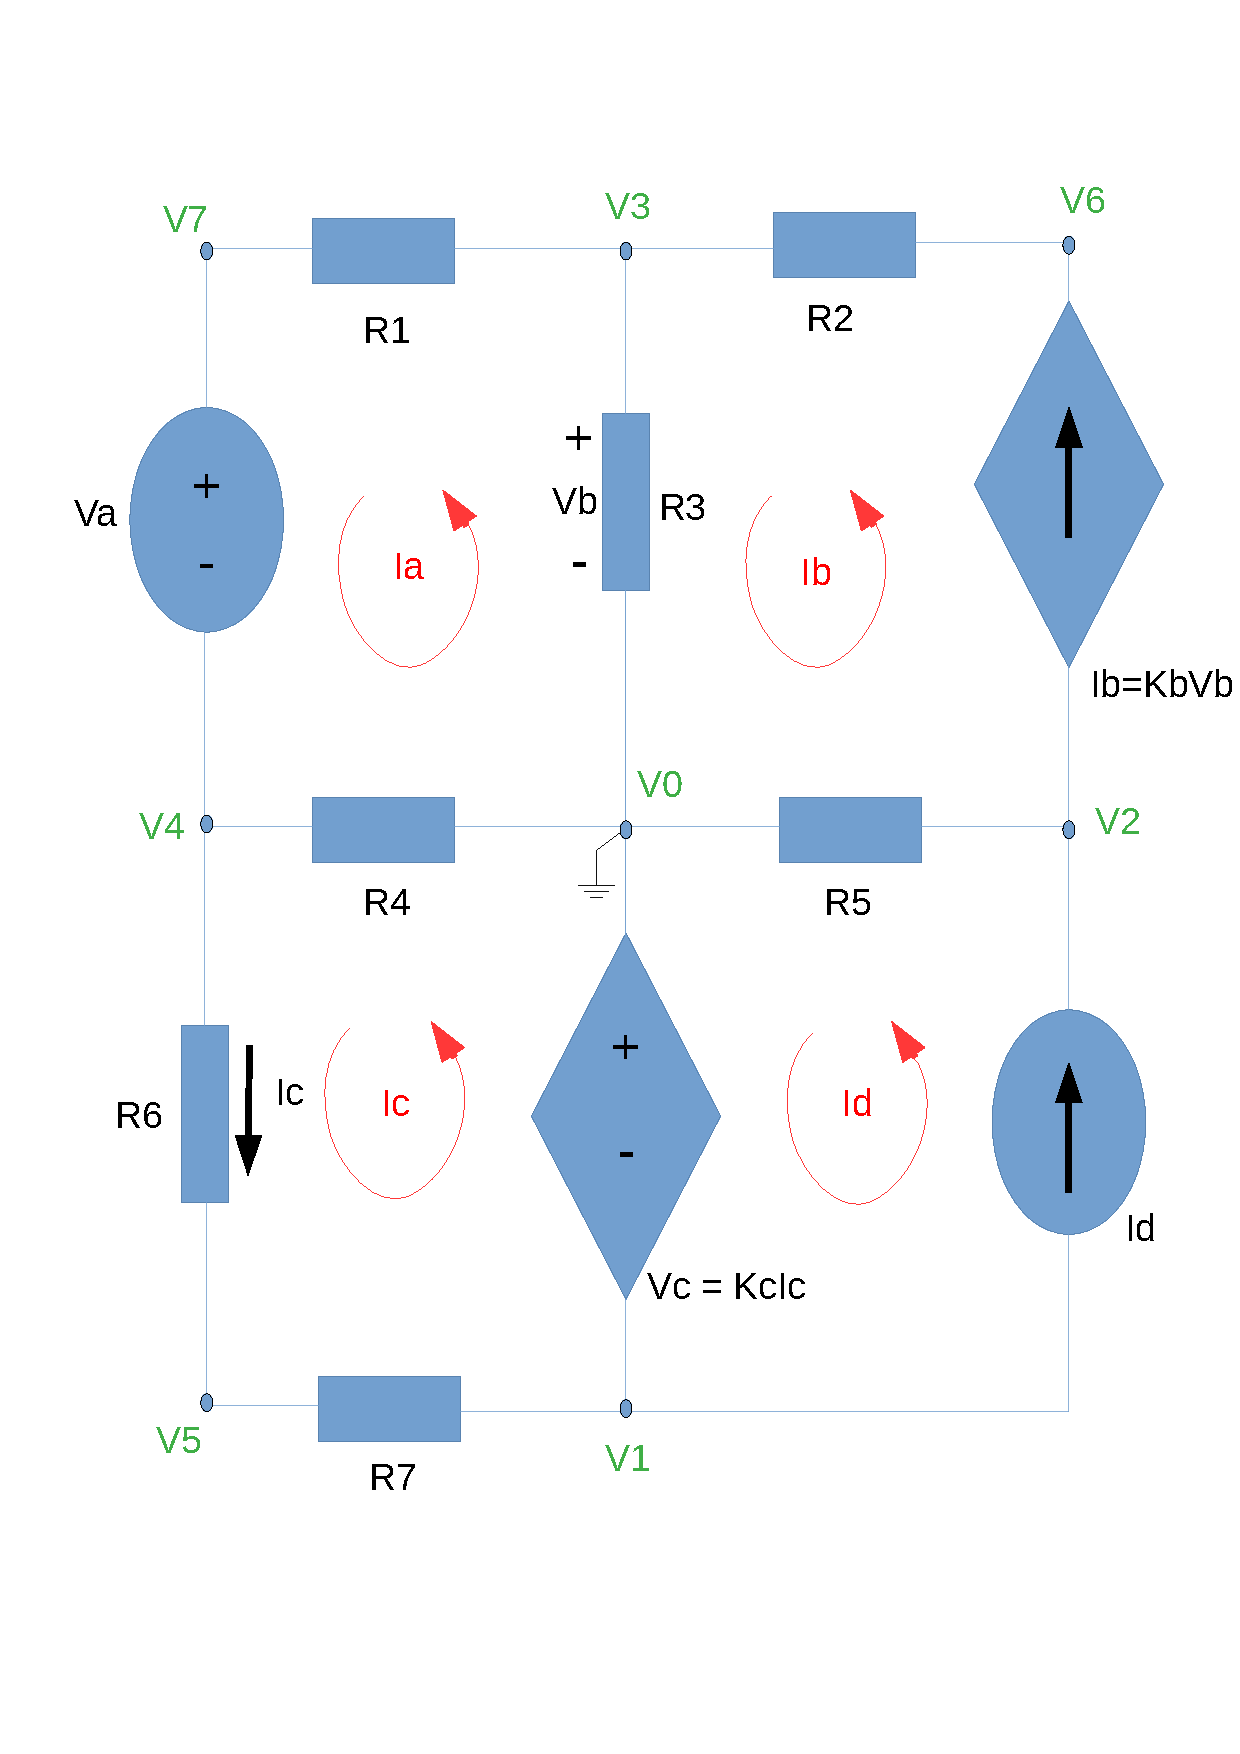
\includegraphics[width=0.4\linewidth]{circuito_tcfe.pdf}
    \caption{Voltage driven serial RC circuit.}
    \label{fig:rc}
\end{figure}



\section{Theoretical Analysis}
\label{sec:analysis}

In this section, the circuit shown in Figure~\ref{fig:circuit} is analysed
theoretically, in terms of voltages and currents in each node and branches respectively.


\section{Nodal Method}

When using the nodal method, we started by defining the 5 essential nodes identified in Figure~\ref{fig:circuit} as $V_0$-$V_5$. The central node $V_0$ was assumed to be the reference 0V, to simplify the expressions as most as possible.
Then we write four equations using KCL for the nodes and Ohm's Law, as well as the dependent sources definitions, so that we arrive at the following linear set of equations, in matrix form:

%b = [Id; -Va/R1; Va/R1; Id]

\[
  \begin{bmatrix}
    0                   & \frac{1}{R_5} & K_b                                 & 0                                              \\
    0                   & 0             & K_b - \frac{1}{R_1} - \frac{1}{R_3} & \frac{1}{R_1}                                  \\
    \frac{1}{R_6 + R_7} & 0             & \frac{1}{R_1}                       & -\frac{1}{R_4}-\frac{1}{R_1}-\frac{1}{R_6+R_7} \\
    -\frac{1}{K_c}      & \frac{1}{R_5} & \frac{1}{R_3}                       & \frac{1}{R_4}
  \end{bmatrix}
  \begin{bmatrix}
    V_1 \\ V_2 \\ V_3 \\ V_4
  \end{bmatrix}
  =
  \begin{bmatrix}
    I_d \\ -\frac{V_a}{R_1} \\ \frac{V_a}{R_1} \\ I_d
  \end{bmatrix}
\]

\hfill


An Octave script was prepared to solve this system numerically. The results are shown in Table \ref{tab:op_nodal_tab}.

\begin{table}[b]
  \centering
  \begin{tabular}{|l|r|}
    \hline
    {\bf Name} & {\bf Value [A or V]} \\ \hline
    \input{op_nodal_tab}
  \end{tabular}
  \caption{Results of Nodal Analysis. A variable that begins  with \textit{I} names a \textit{current} in \textit{Ampere}; the ones that start with \textit{V} name a \textit{voltage} in \textit{Volt} }
  \label{tab:op_nodal_tab}
\end{table}



\section{Mesh Method}

By analysing the circuit in terms of the meshes, we started by assuming that we have $4$ unknown quantities: $I_a, I_b, I_c, I_d$ (four meshes).
Effortlessly, we realized that the current in the mesh of the lower right corner is defined by the current source $I_d$.
Using the fact that the voltage-controlled current source presented in the mesh of $I_b$ only belongs to this mesh and that $I_b = K_b V_b$ (formula developed in \ref{restrict1}), there is no need in writing an equation for the loop of current $I_b$.
As a result, we are left with 2 independent variables: $I_b$ and $I_c$ and the following equations:


%equations
\begin{equation}
  (R_1 + R_2 + R_4) \frac{K_b R_3 -1}{K_b R_3}I_b  - R_3I_b  - R_4I_c = -Va
  \label{mesh1}
\end{equation}

\begin{equation}
  -R_4 \frac{K_b R_3 - 1}{K_b R3}I_b + (R_4  + R_6 + R_7 - K_c)I_c = 0
  \label{mesh2}
\end{equation}

During the derivation of the previous equations, the next restrition equations were used:

\begin{equation}
  I_a = \frac{K_b R_3 -1}{K_b R_3} I_b
  \label{restrict1}
\end{equation}

\begin{equation}
  V_c = K_c I_c
  \label{restrict2}
\end{equation}

By solving equations with a script of \textit{Octave}, we got the following results presented in the table \ref{tab:op_mesh_tab}

From knowing the current of the meshes, we compute the currents and  potencial values in each branch and node respectively, by keeping in mind that was used the same reference node $V_0$.


%signals-------------------->
\begin{table}[h]
  \centering
  \begin{tabular}{|l|r|}
    \hline
    {\bf Name} & {\bf Value [A or V]} \\ \hline
    \input{op_mesh_tab}
  \end{tabular}
  \caption{Results of Mesh Analysis. A variable that begins  with \textit{I} names a \textit{current} in \textit{Ampere}; the ones that start with \textit{V} name a \textit{voltage} in \textit{Volt}}
  \label{tab:op_mesh_tab}
\end{table}


%\lipsum[1-1]




\section{Simulation Analysis}
\label{sec:simulation}

\subsection{Operating Point Analysis}

Table~\ref{tab:op} shows the simulated operating point results for the circuit
under analysis. Compared to the theoretical analysis results, one notices the
following differences: describe and explain the differences.

\begin{table}[h]
  \centering
  \begin{tabular}{|l|r|}
    \hline    
    {\bf Name} & {\bf Value [A or V]} \\ \hline
    @gib[i] & -2.65517e-04\\ \hline
@id[current] & 1.025904e-03\\ \hline
@r1[i] & -2.53670e-04\\ \hline
@r2[i] & -2.65517e-04\\ \hline
@r3[i] & -1.18476e-05\\ \hline
@r4[i] & 1.220737e-03\\ \hline
@r5[i] & -1.29142e-03\\ \hline
@r6[i] & 9.670671e-04\\ \hline
@r7[i] & 9.670671e-04\\ \hline
v(1) & -7.95657e+00\\ \hline
v(2) & 3.950179e+00\\ \hline
v(3) & -3.64391e-02\\ \hline
v(4) & -4.95541e+00\\ \hline
v(5) & -6.94792e+00\\ \hline
v(6) & -5.78231e-01\\ \hline
v(7) & 2.284139e-01\\ \hline
v(8) & -4.95541e+00\\ \hline

  \end{tabular}
  \caption{Operating point. A variable preceded by @ is of type {\em current}
    and expressed in Ampere; other variables are of type {\it voltage} and expressed in
    Volt.}
  \label{tab:op}
\end{table}

\lipsum[1-1]


\subsection{Transient Analysis}

Figure~\ref{fig:trans} shows the simulated transient analysis results for the
circuit under analysis. Compared to the theoretical analysis results, one
notices the following differences: describe and explain the differences.

\begin{figure}[h] \centering
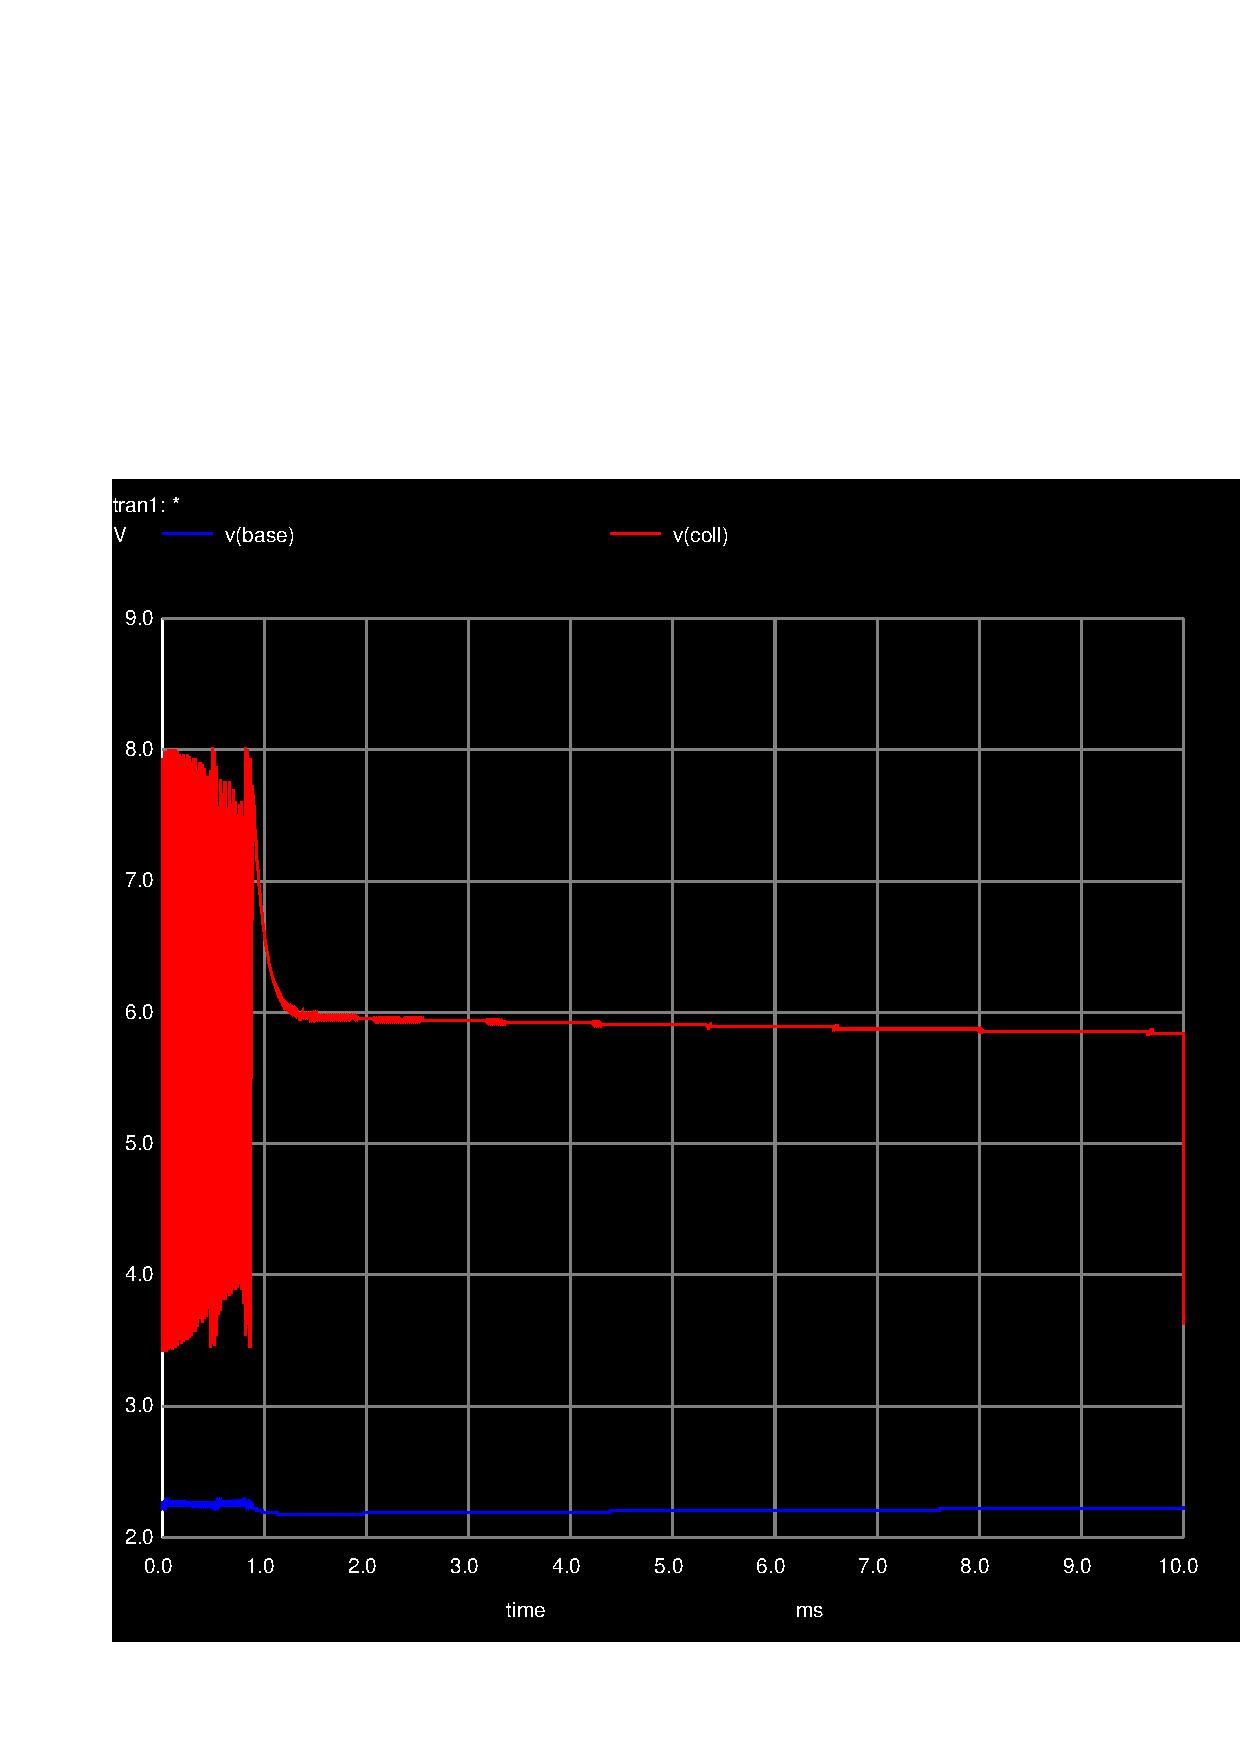
\includegraphics[width=0.6\linewidth]{trans.pdf}
\caption{Transient output voltage}
\label{fig:trans}
\end{figure}

\lipsum[1-1]



\subsection{Frequency Analysis}

\subsubsection{Magnitude Response}

Figure~\ref{fig:acm} shows the magnitude of the frequency response for the
circuit under analysis. Compared to the theoretical analysis results, one
notices the following differences: describe and explain the differences.

\begin{figure}[h] \centering
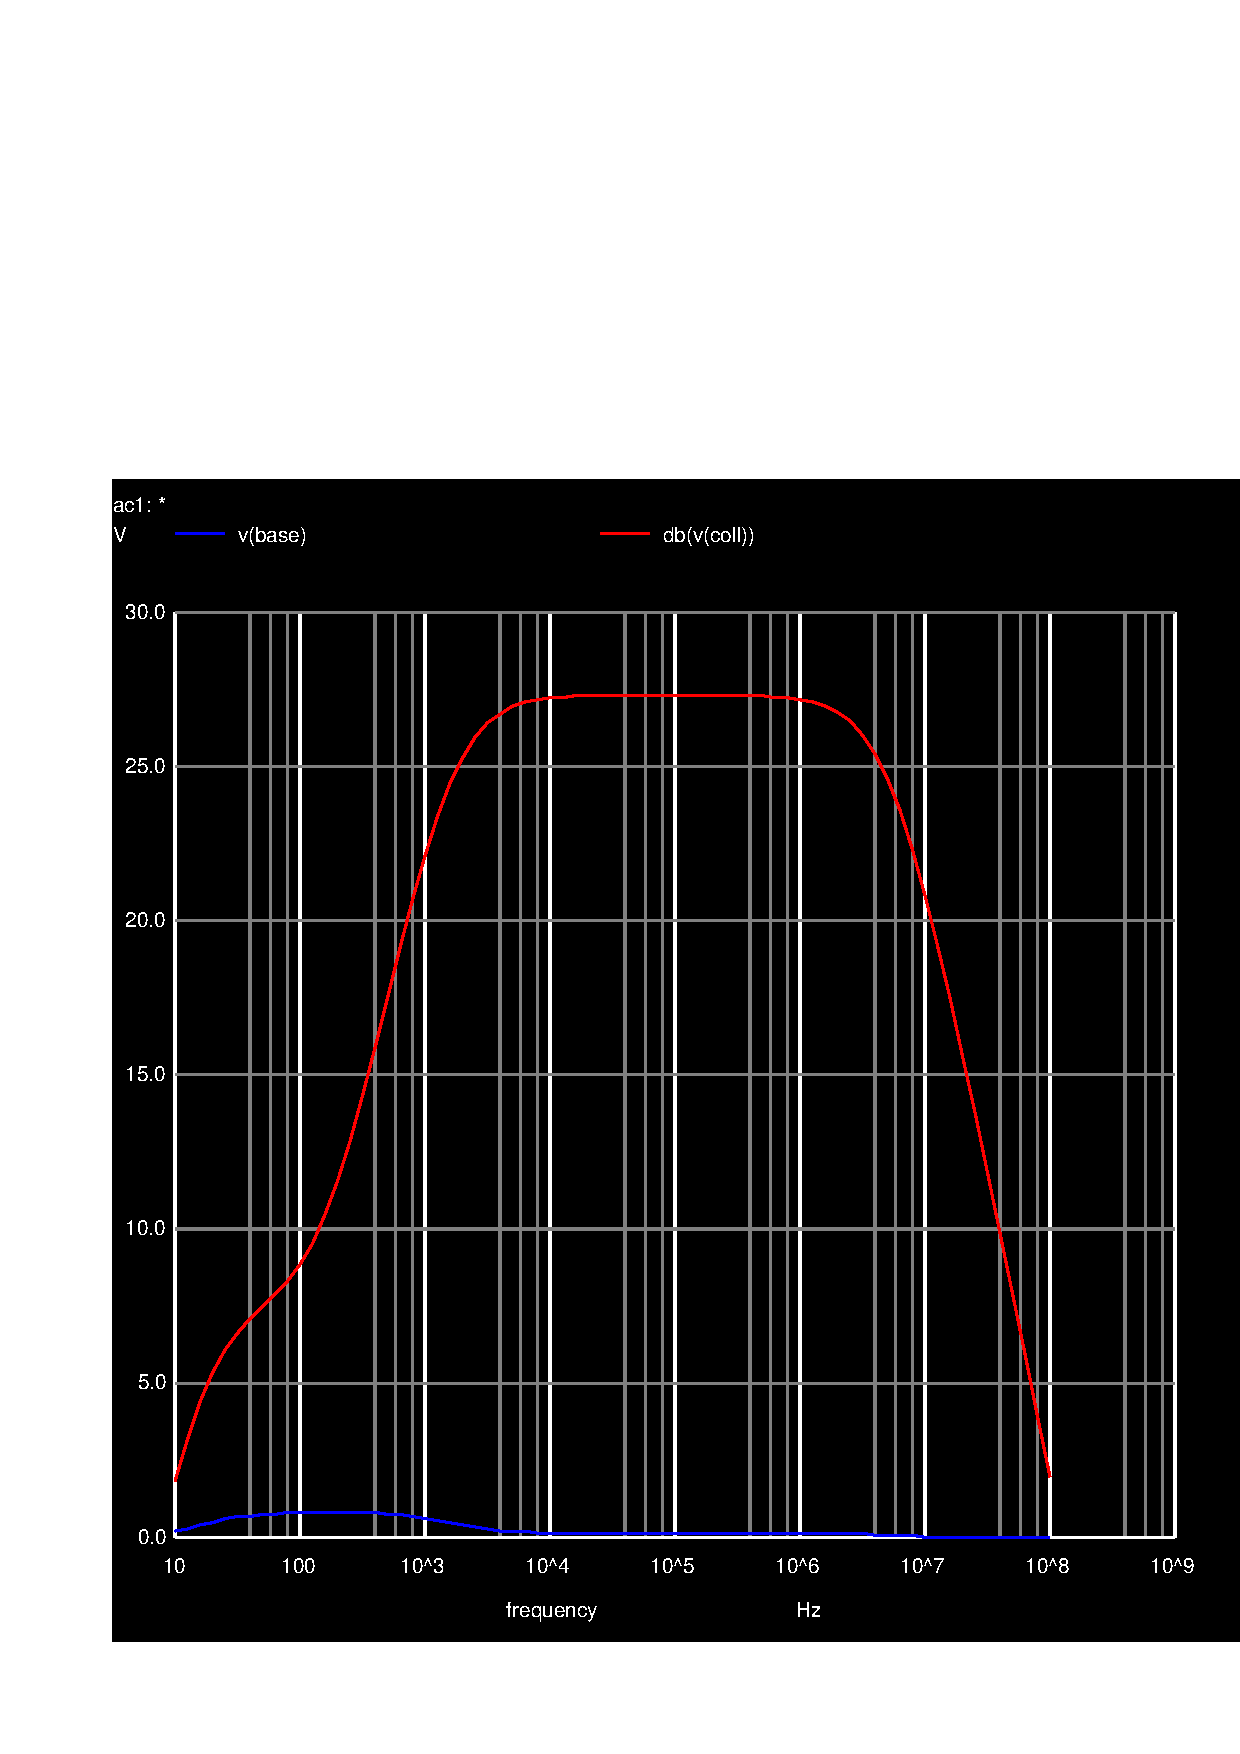
\includegraphics[width=0.6\linewidth]{acm.pdf}
\caption{Magnitude response}
\label{fig:acm}
\end{figure}

\lipsum[1-1]

\subsubsection{Phase Response}

Figure~\ref{fig:acp} shows the magnitude of the frequency response for the
circuit under analysis. Compared to the theoretical analysis results, one
notices the following differences: describe and explain the differences.

\begin{figure}[h] \centering
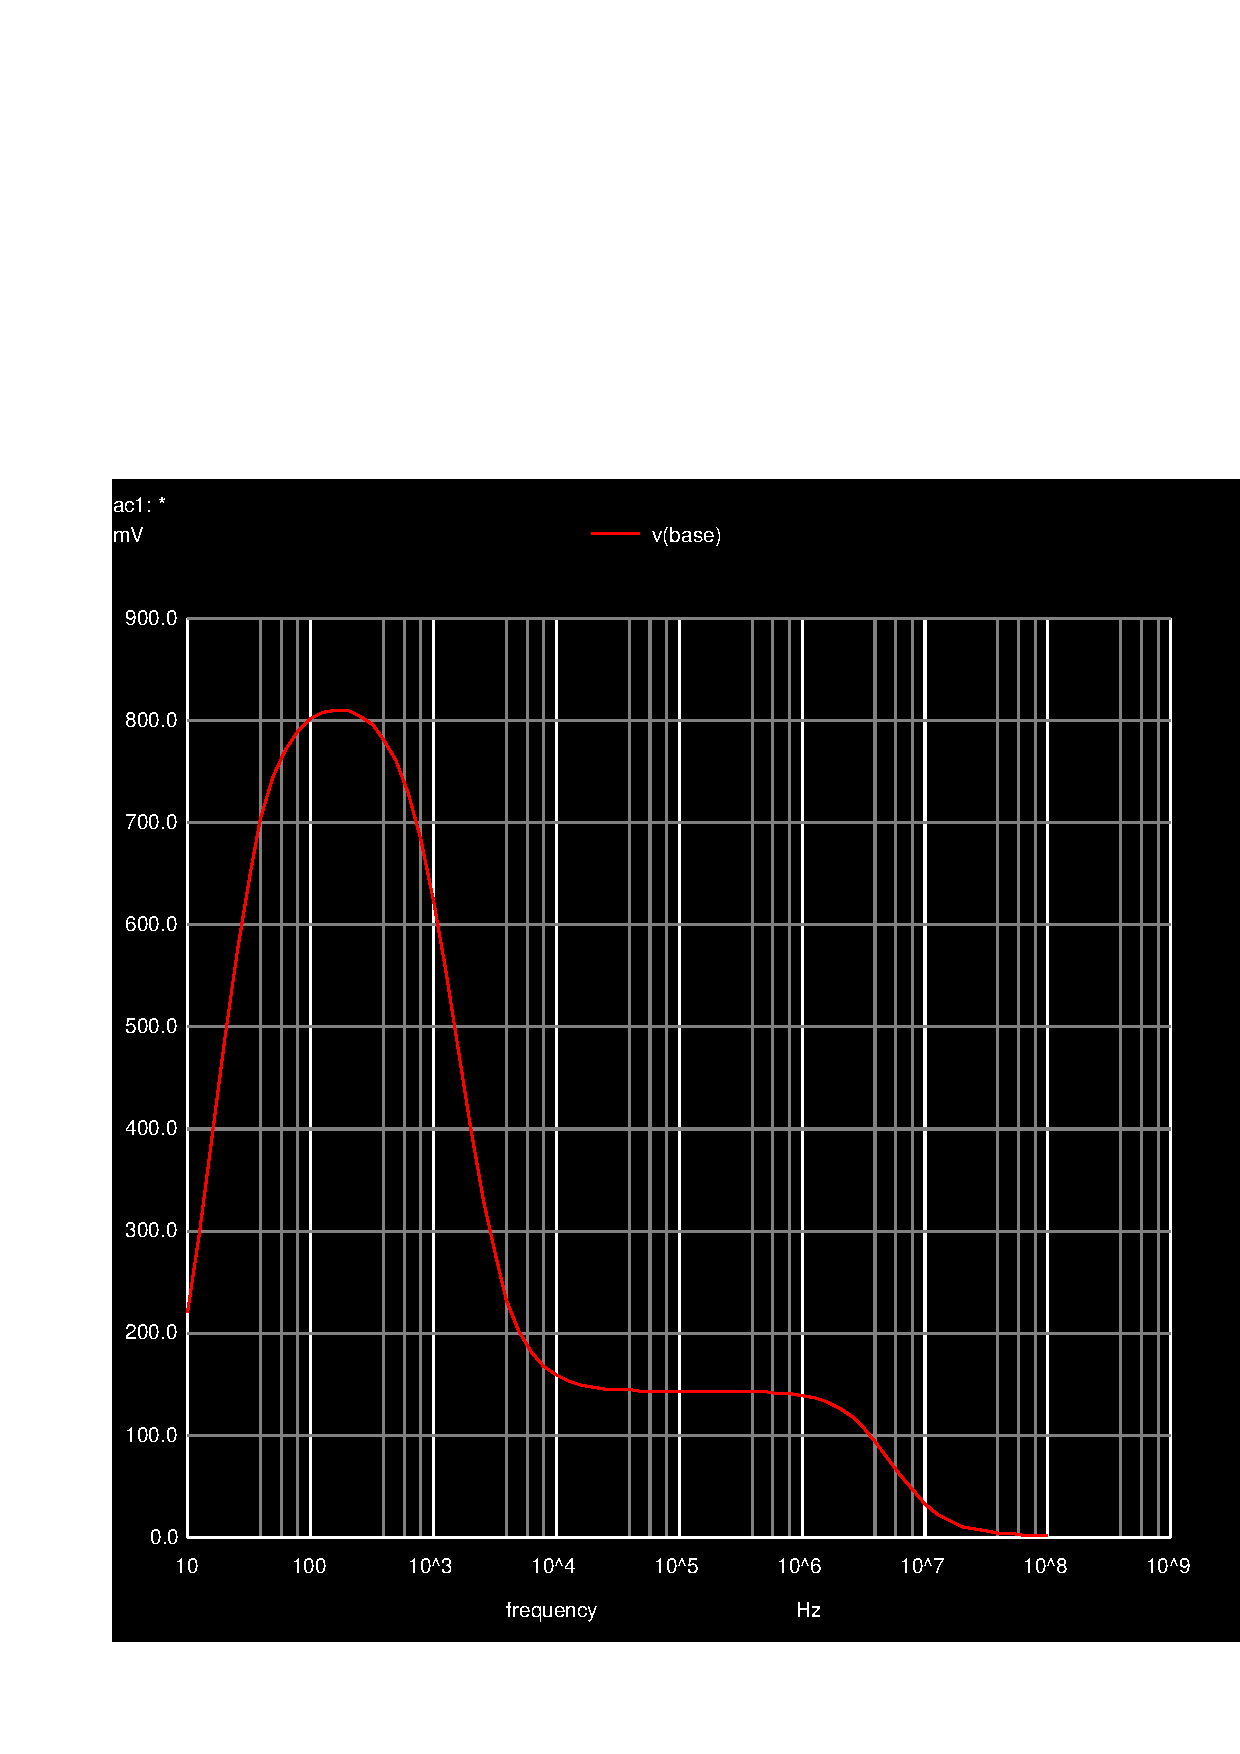
\includegraphics[width=0.6\linewidth]{acp.pdf}
\caption{Phase response}
\label{fig:acp}
\end{figure}

\lipsum[1-1]

\subsubsection{Input Impedance}

Figure~\ref{fig:zim} shows the magnitude of the frequency response for the
circuit under analysis. Compared to the theoretical analysis results, one
notices the following differences: describe and explain the differences.

\begin{figure}[h] \centering
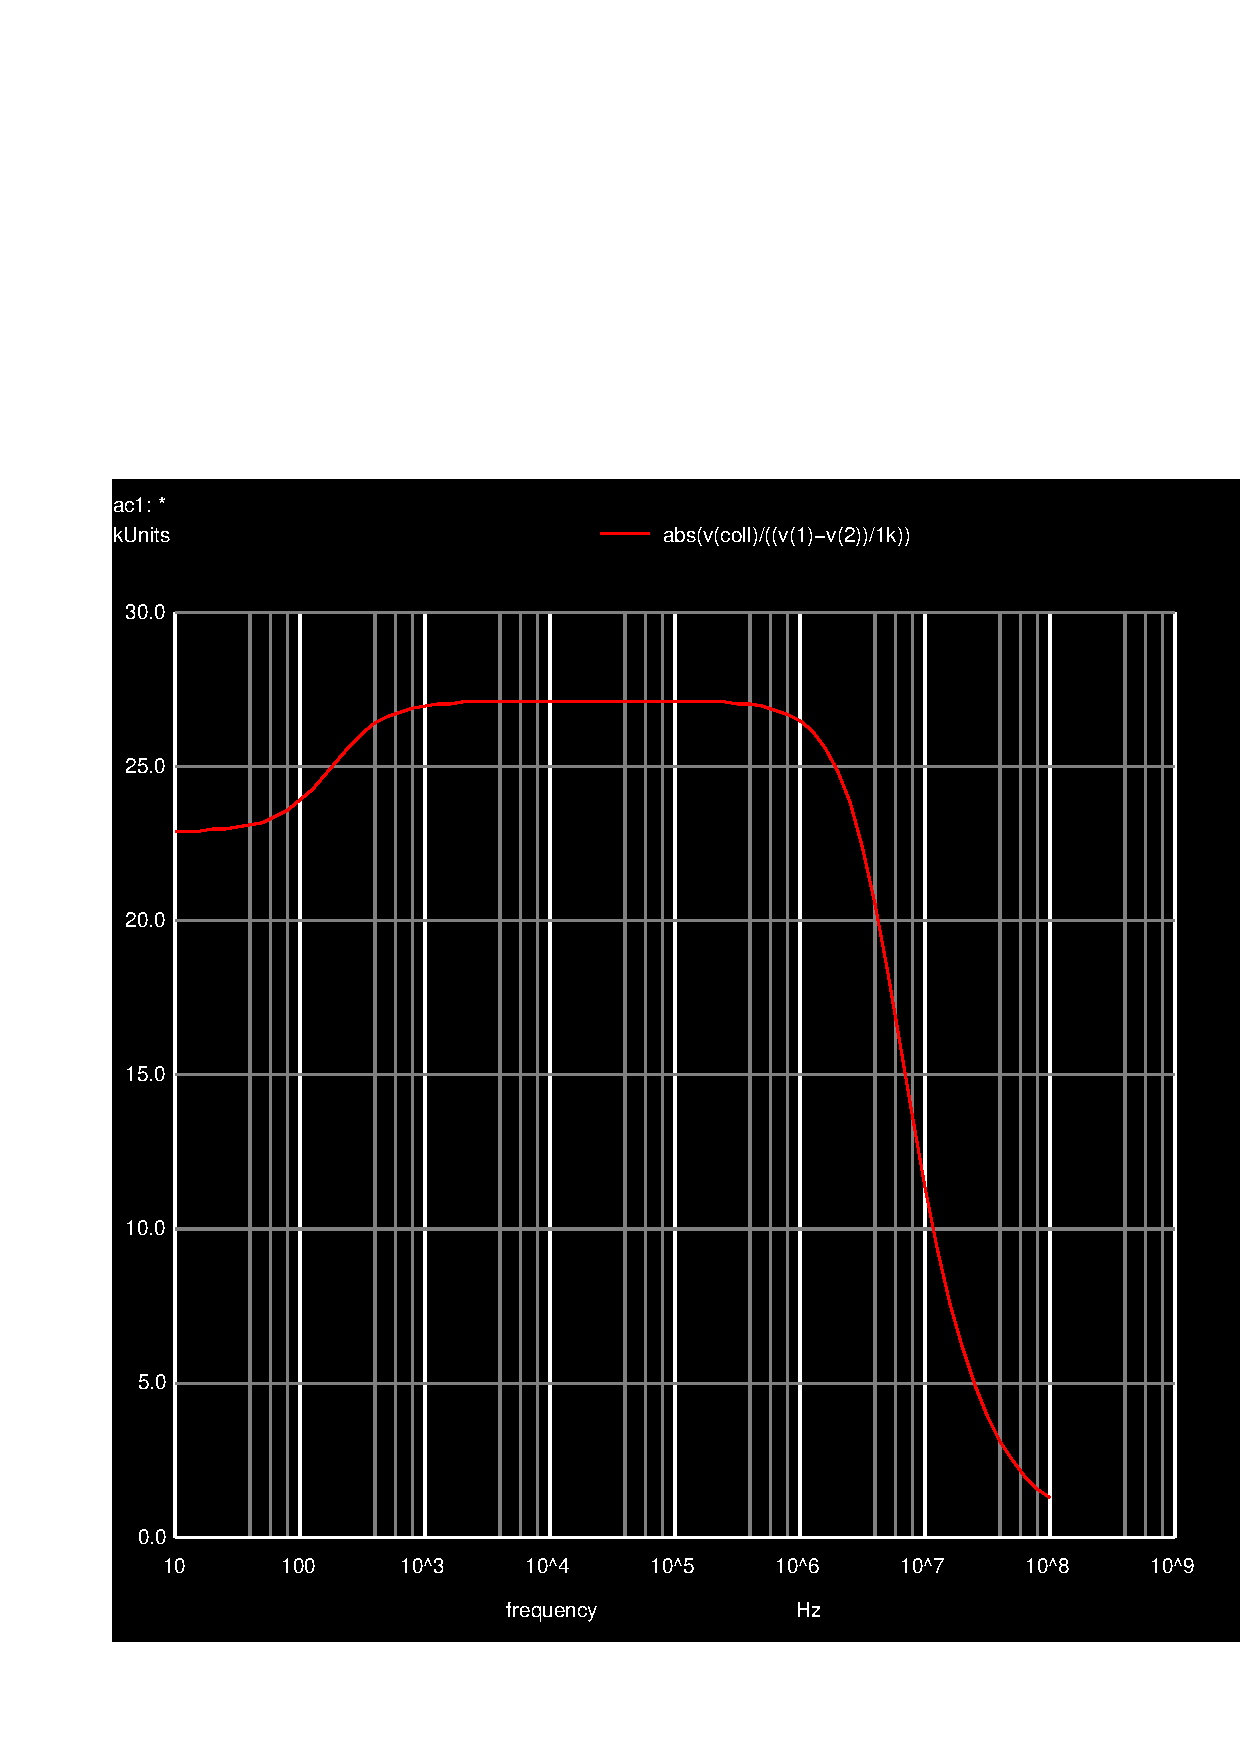
\includegraphics[width=0.6\linewidth]{zim.pdf}
\caption{Input impedance}
\label{fig:zim}
\end{figure}

\lipsum[1-1]





\section{Side by side comparison}
\label{sec:comparison}

In this section we compare both results side by side. Firstly, the output of the envelope detector (take note that the theoritcal analysis one is the plot in orange):
\begin{figure}[h]
    \centering
    \begin{subfigure}{0.23\textwidth}
        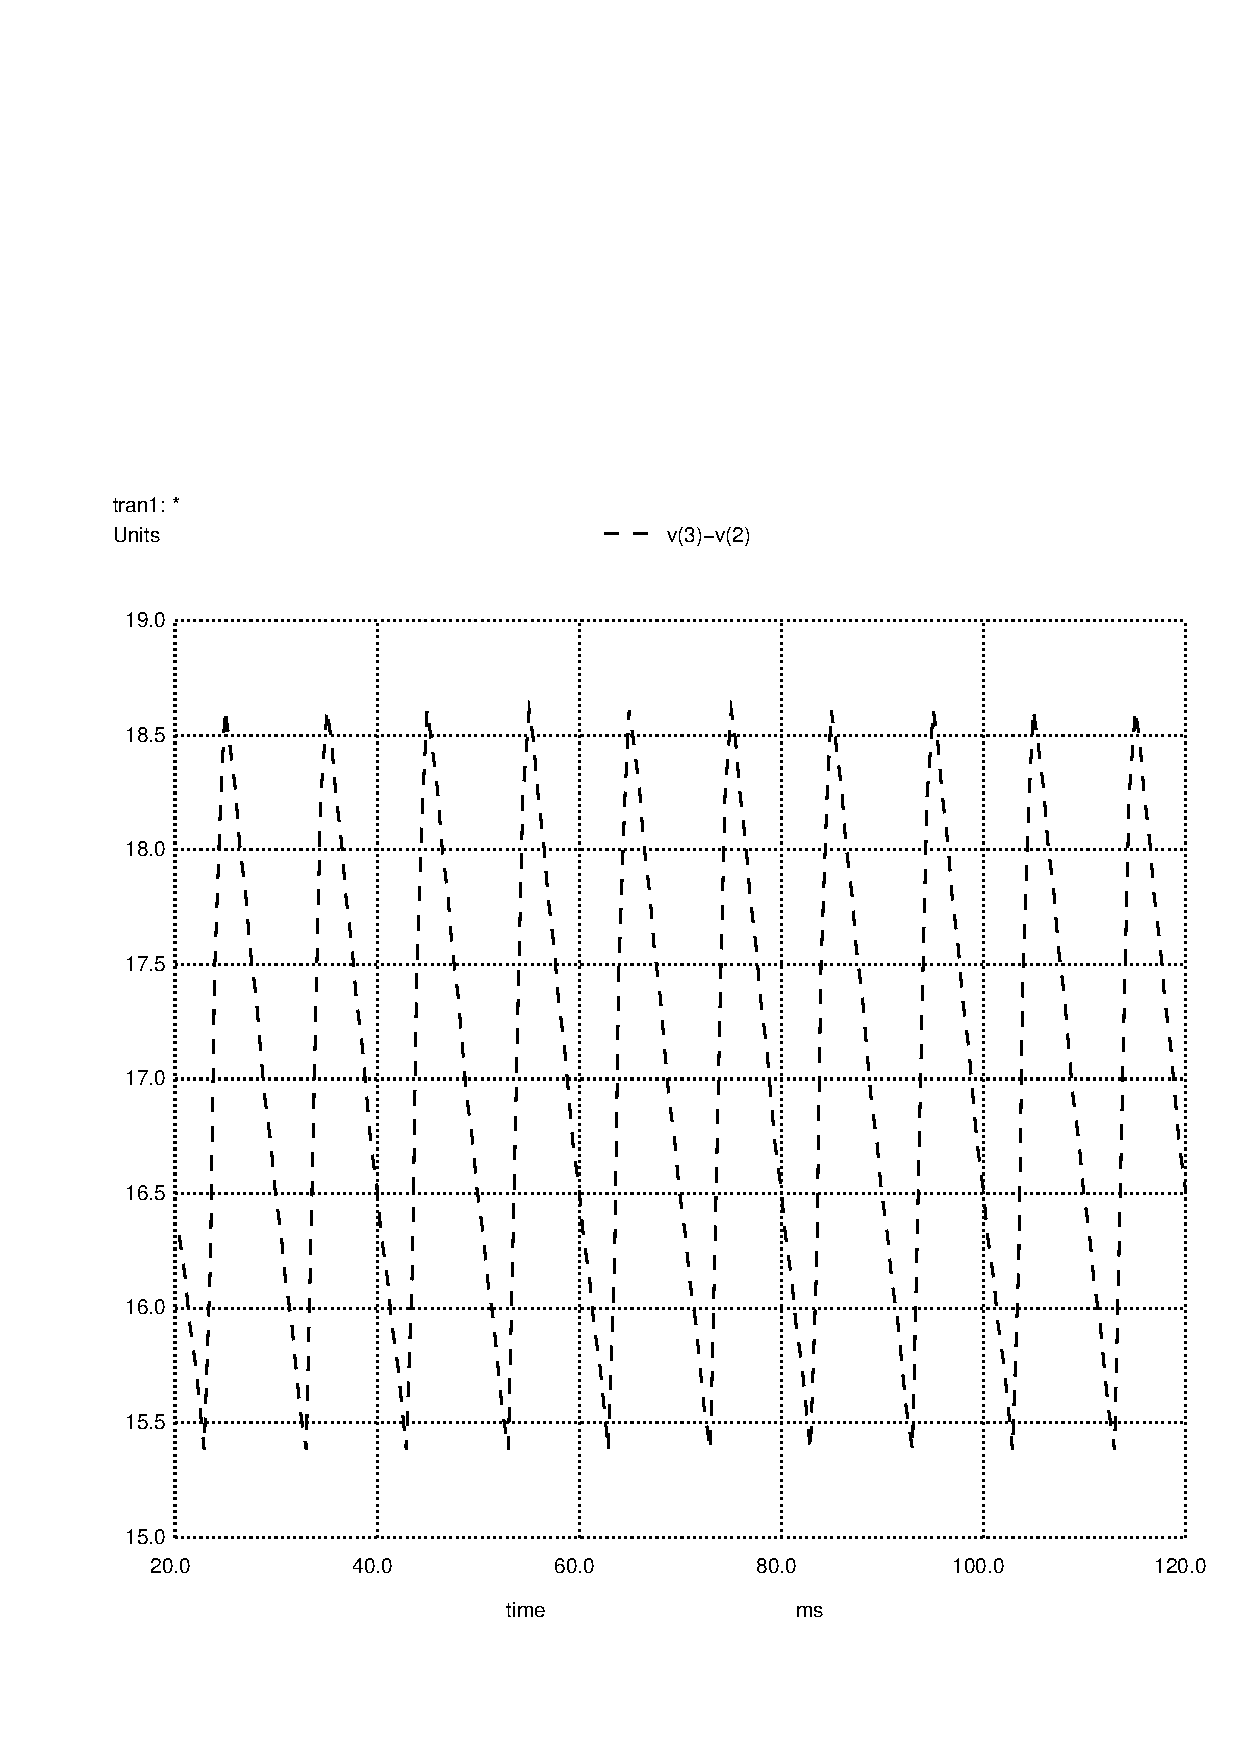
\includegraphics[width=\linewidth, clip]{solution2.pdf}
        \label{fig:envd1}
    \end{subfigure}
    \begin{subfigure}{0.23\textwidth}
        \includegraphics[width=\linewidth, clip]{venvlope.eps}
        \label{fig:envd2}
    \end{subfigure}
    \caption{\small Envelope detector output (left - simulation; right - theoretical )}
    \label{env_detector}
\end{figure}

\begin{figure}[h]
    \centering
    \begin{subfigure}{0.23\textwidth}
        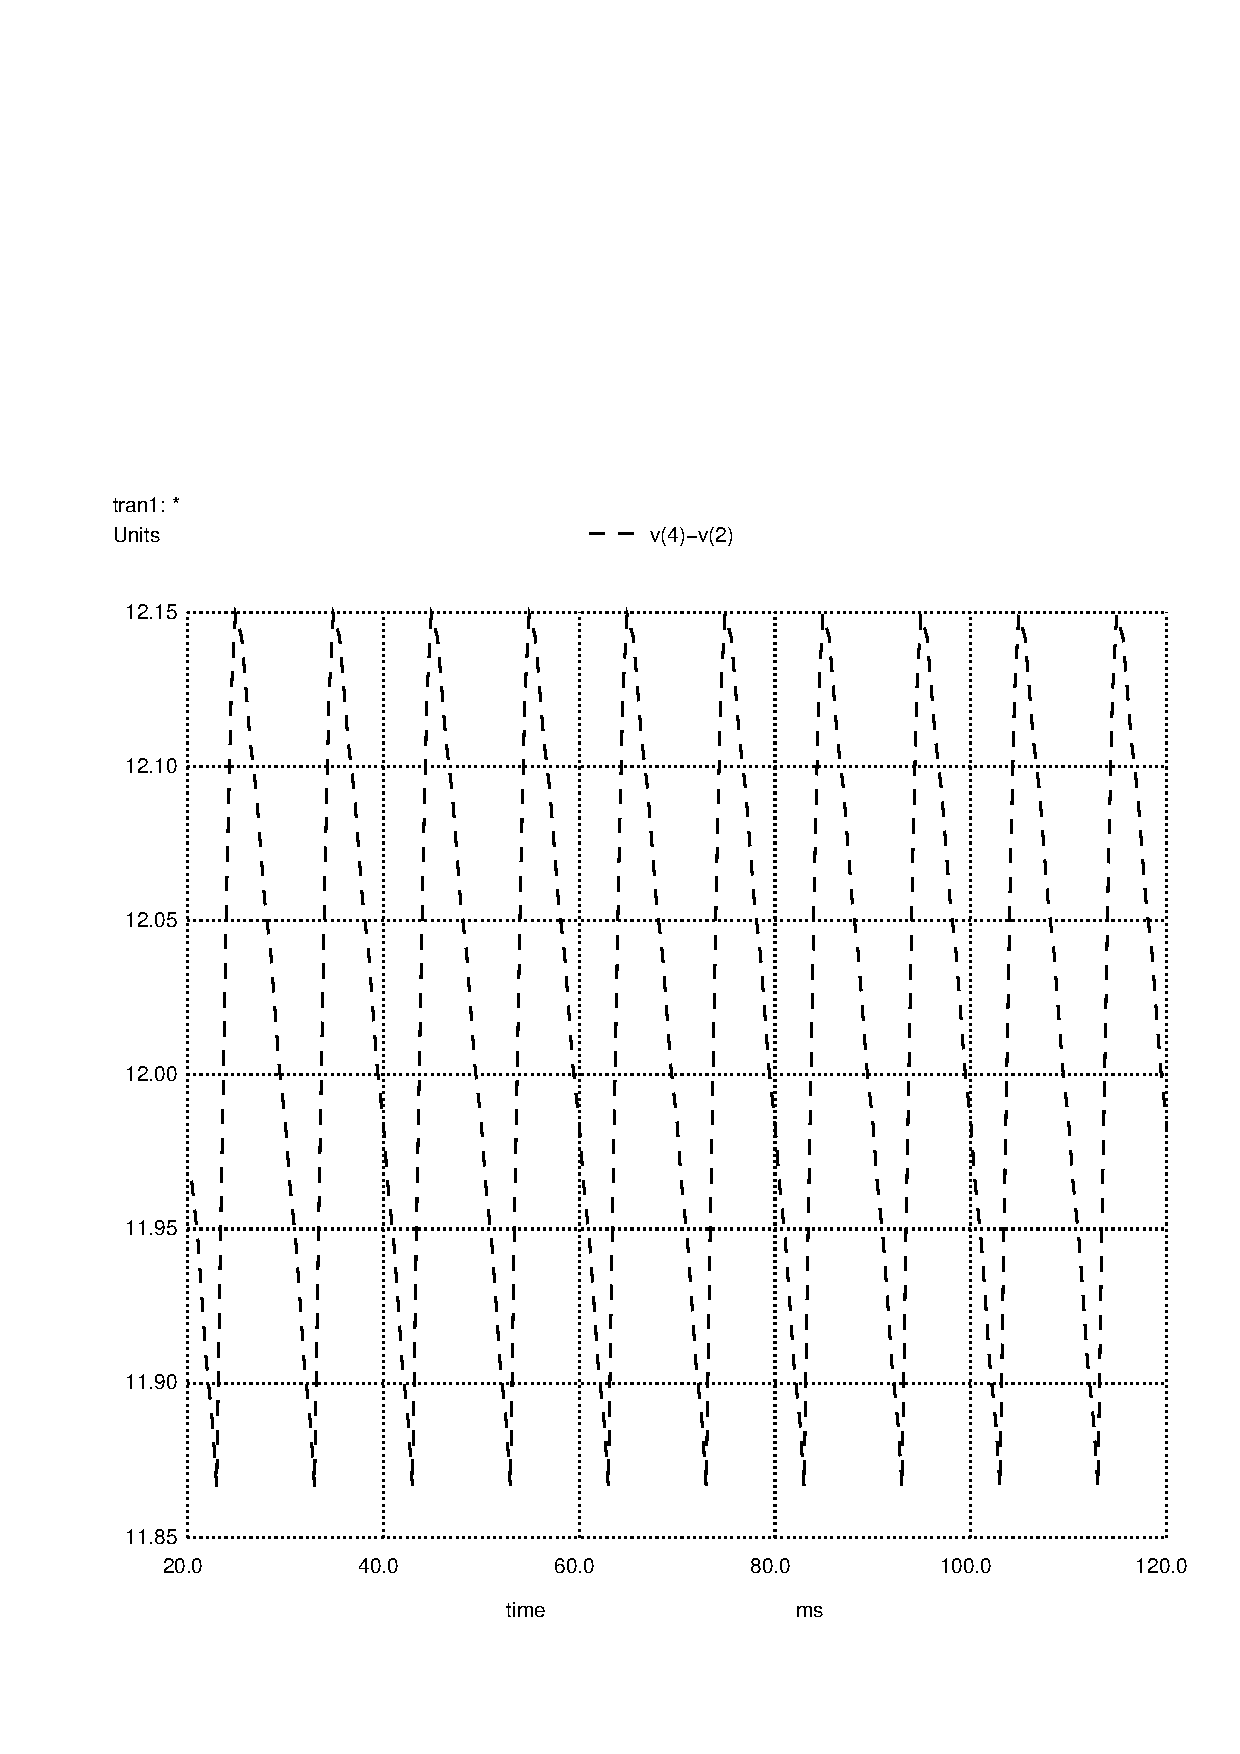
\includegraphics[width=\linewidth, clip]{solution1.pdf}
        \label{fig:voltr1}
    \end{subfigure}
    \begin{subfigure}{0.23\textwidth}
        \includegraphics[width=\linewidth, clip]{voltageRegulator.eps}
        \label{fig:voltr2}
    \end{subfigure}
    \caption{\small Voltage regulator output (left - simulation; right - theoretical )}
    \label{volt_reg}
\end{figure}

The shape of the graphs, both envelope detector and voltage regulator is similar, so we can concluse that both fullfill their purposes and the theoretical model used was good at predicting the general behaviour of the circuit. 
However, especially on the voltage regulator graphs, we can see some differences in the scale of the oscillations, that can be due to the different models used in our theoretical simulation, compared to ngspice.
We will quantify this difference later in the difference of the ripple in both simulations.

\begin{figure}[h]
    \centering
    \begin{subfigure}{0.23\textwidth}
        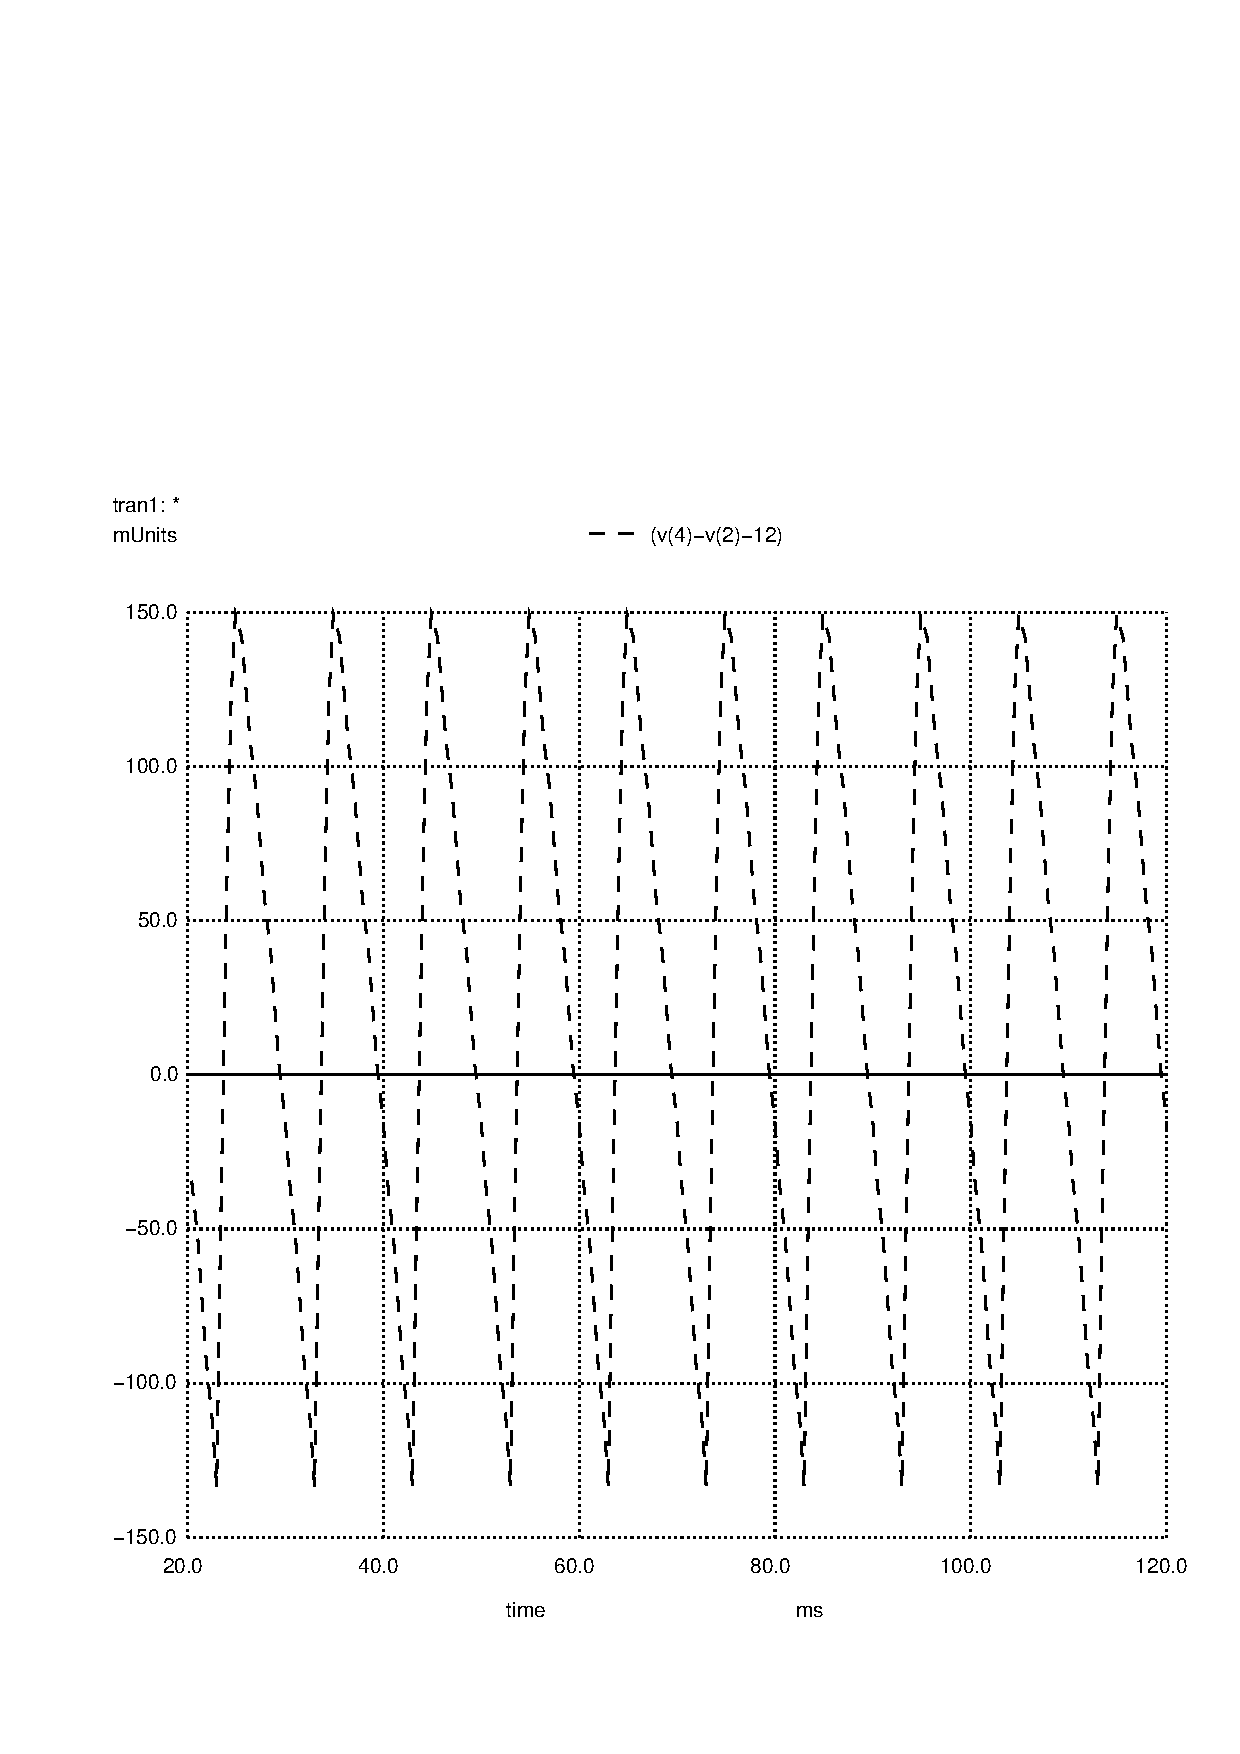
\includegraphics[width=\linewidth, clip]{solution12.pdf}
        \label{fig:output1}
    \end{subfigure}
    \begin{subfigure}{0.23\textwidth}
        \includegraphics[width=\linewidth, clip]{Deviation.eps}
        \label{fig:output2}
    \end{subfigure}
    \caption{\small $V_Out - 12$ - measure of the output DC deviation + AC component (left - simulation; right - theoretical )}
    \label{output_deviation}
\end{figure}

Once again, as in the previous graphs, the output deviation graph has a similar shape but a noticeable difference in scale, probably due to different models.



\section{Conclusion}
\label{sec:conclusion}


The ultimate goal of this laboratory assignment, to analyse
the given circuit theoretically and using simulation (and consequently
familiarising the group with the tools used), has been achieved, since
the simulation results matched the theoretical results with great accuracy.
These results were expected because we use the same linear models to
describe the behaviour of the components in \textit{Ngspice} and in
theoretical analysis (\ref{sec:analysis}). Furthermore, none of
the components is time dependent.

%\lipsum[1-1]

%\cleardoublepage

% ----------------------------------------------------------------------
%  Bibliography
% ----------------------------------------------------------------------
%\addcontentsline{toc}{section}{\bibname}
%\bibliographystyle{abbrvunsrtnat} % <<<<< SELECT IF USING REFERENCES BY NUMBER (CITATION ORDER)
%\bibliography{../../../BIBfile.bib}

% ----------------------------------------------------------------------
\end{document}
% ----------------------------------------------------------------------

